%%%%%%%%%%%%%%%%%%%% icsc2026_evoking_harmony_4p_v2.tex %%%%%%%%%%%%%%%%%%%%%
% Short (4-page) slide-aligned variant. Does not replace icsc2026_evoking_harmony_4p.tex.

\documentclass[runningheads,a4paper]{llncs}
\usepackage{icsc2026_submission}
\usepackage{url}
\usepackage{amsmath}
\usepackage{graphicx}
\usepackage{hyperref}
\hypersetup{hidelinks}
\newcommand{\keywords}[1]{\par\addvspace\baselineskip
\noindent\keywordname\enspace\ignorespaces#1}

\pagestyle{headings}

\begin{document}

\mainmatter

\title{Evoking Harmony via Convolution}
\titlerunning{Evoking Harmony}
\author{\submissionauthor}
\authorrunning{\submissionauthorrunning}
\institute{\submissioninstitute}

\maketitle

\begin{abstract}
I show how to evoke the pitch-class content of a chord from an arbitrary
source by convolving it with a short impulse response whose grains lie on
those pitch-classes in every octave. A Csound implementation
(\texttt{chord\_convolver}) builds one joint IR with
frequency-dependent grain length, equal-energy normalization across octaves,
inverse A-weighting, a dry Dirac, and a single \texttt{ftconv}. I contrast the effect with a linear comb and a generic
constant-$Q$ bank, and demonstrate it on a twilight field recording alongside Ch\^{a}teau de
Lagarde.
\keywords{csound, harmony, convolution, constant-$Q$, field recording}
\end{abstract}

\section{Introduction}

As a boy crossing the desert at night I heard melodies and chords in the wind
outside my father's car. This paper reports Csound~\cite{csound_home} experiments that
evoke such harmonies from varied sources by convolving a signal with an
impulse response whose grains occupy the pitch-classes of a chosen chord on every
octave. Materials are in \submissionmaterialsrepo.

The effect sits at the boundary of timbre and tonality, against a long-standing
disjunction between ``non-tonal'' electroacoustic practice (acousmata) and
tonal practice (pitch relations abstracted from actual sounds). That split
goes back to the 1950s--1960s mix of technological utopianism and musical
serialism. A constant-$Q$ bank \emph{centered on those pitch-classes} is
closely related; a generic constant-$Q$ tiling is only loosely related; a comb
filter is less related still (periodic in linear Hz); Gabor/Morlet cells not
centered on pitch-classes are a poor fit.

\section{Mathematics}

A \emph{grain} is one windowed sinusoid (pitch-class $c$, octave $n$). Its
frequency response is a \emph{kernel} $H_{c,n}$. The \emph{impulse response}
is the sum of the loudness-balanced grains plus a Dirac, then jointly
$\ell_2$-normalized. For a chord $C$ those kernels form an octave-related
scaled family:
\[
H_C(f)=\sum_{c\in C}\sum_n H_{c,n}(f),\qquad
H_{c,n}(f)\simeq H_c(2^{-n}f).
\]
With $u=\log_2 f$, octave shift is unit translation and
$H_C(u+1)\simeq H_C(u)$: the chord is the unit cell of a log-periodic filter.
Grain length
\[
T(f)=\min\bigl(T,\,T\cdot 440/f\bigr)
\]
is constant-$Q$ above $440\,\mathrm{Hz}$; below the pivot, duration is capped
at $T$~\cite{gabor1946theory}.

\section{Method}

\texttt{chord\_convolver} selects MIDI notes whose pitch-classes are
in $C$ (reduced modulo 12; negatives unused) and assigns each partial $f$ a
causal half-cosine of length $T(f)$, with $T$ clamped to
$[0.01,1.5]\,\mathrm{s}$ (starts at $1$, fades to $0$). Grains are levelled by octave, a
Dirac is added at sample~$0$, the IR is jointly $\ell_2$-normalized, and
\texttt{ftconv}~\cite{csoundmanualftconv} is applied once. Full signatures and
code are in \submissionmaterialsrepocite.

Both the causal window and the cap on $T(f)$ serve auditory fusion. Since
$Y(f)=H(f)X(f)$ vanishes wherever the source has no energy, the lattice can only
expose pitch content the source already contains; what makes that content read
as latent in the source rather than as an added voice is keeping the harmonic
response inside the source's own events, since energy persisting after the
source falls silent would be a cue for a separate resonating object. On a
$50\,\mathrm{ms}$ impulse response driven by a $3\,\mathrm{Hz}$ impulse train,
this design leaves under $3\,\%$ of each period's energy outside the interval
the dry source occupies, against a third or more for an uncapped or
symmetrically windowed grain.

Levelling the octaves takes two stages. Considering a source as broadband, the
output power contributed by partial $k$ is $S_0 E_k$ by Parseval's theorem, so
equal presence requires equal grain \emph{energy}, giving
$A(f)\propto T(f)^{-1/2}$; a constant factor holds total grain energy fixed so
the impulse and Dirac gains keep their meaning. Loudness tracks power rather
than spectral density because every grain occupies less than one auditory
filter---at most $0.74$ of an ERB~\cite{glasberg1990derivation}. Normalizing the
window integral instead, which fixes peak transfer gain, tilts the lattice
bright by some $8\,\mathrm{dB}$, because the grain bandwidth $\approx 1/T(f)$
widens as the window shortens. The second stage is inverse IEC A-weighting
(shelf at $150\,\mathrm{Hz}$, boost capped at $+6\,\mathrm{dB}$), which turns
equal power into approximately equal loudness. Equalizing critical bands rather than
partials, which attenuates the crowded low octaves by 4 to $6\,\mathrm{dB}$, is
available as an option but is not used here (compensation 1; no ERB
correction).

A chord-restricted constant-$Q$ bank is a near neighbour (same lattice,
ongoing IIR filtering). A generic three-semitone constant-$Q$ tiling lacks
chord identity. A comb with delay $1/f_0$ has equal linear-Hz spacing.

\section{Results}

Figure~\ref{fig:spectrograms} compares click and noise under dry, comb
($f_0=200\,\mathrm{Hz}$), sparse CQT (every three semitones), and evoke with
PCs $0,4,7,11$ (CM7), loudness-matched to within $1.1\,\mathrm{dB}$
A-weighted within each source group. Comb is linear-periodic; CQT is
log-periodic but not chordal; the convolver shows the CM7 lattice,
articulated to the top of the audible range under equal-energy normalization.

\begin{figure}[t]
\centering
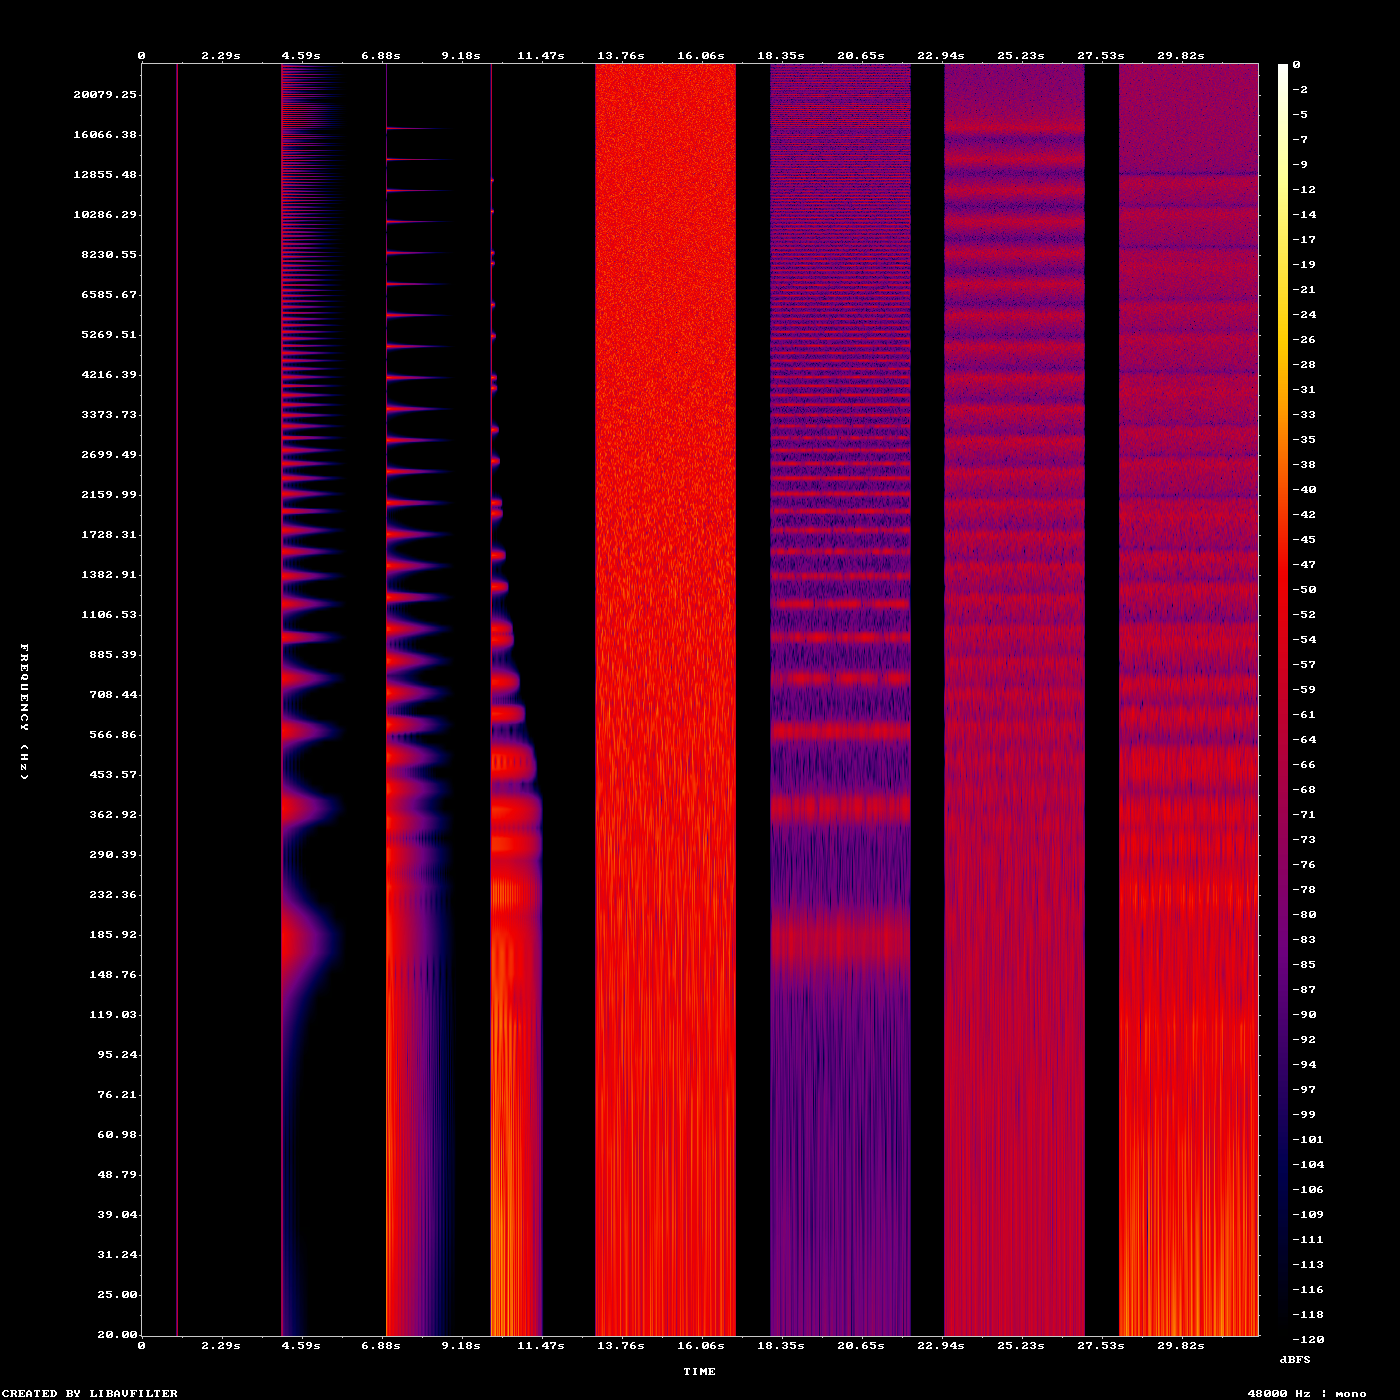
\includegraphics[width=\linewidth,keepaspectratio]{icsc2026_spectrograms.png}
\caption{Log-frequency spectrogram (left to right): dry click; click comb;
click CQT; click evoke CM7; then the same four treatments of noise.}
\label{fig:spectrograms}
\end{figure}

A twilight walk alongside Ch\^{a}teau de Lagarde recorded with a Tascam DR-40 is processed under score
control of $T$, wet/dry, compensation type (here always 1, equal energy), and
pitch-classes (MIDI key numbers, reduced modulo 12)
\submissioncitesoundwalk. Moments include a chord progression within voices,
bells with a subtle effect, bells again with a stronger effect and voices 
following, and \emph{``Bonjour''} with voices following.

\section{Discussion}

Evoking harmony is chord-specific and log-periodic, unlike a comb, and uses
finite causal grains plus a dry Dirac in one impulse response rather than a steady filterbank. It is most
appealing when harmonic sensation remains subtle relative to the source;
wetter settings yield a clearer shadow or ring, or even more abstract harmonic and rhythmic textures. To see more:
\submissiongithubsupplement{} include audio and orchestra code.

\paragraph{Note.}
\submissionainote{}

\bibliographystyle{unsrt}
\bibliography{icsc2026_evoking_harmony_v2}

\end{document}
